% Titre de la partie
\section[Modélisation visuelle]{Affichage et interface avec la modélisation}

%%%%%%%%%%%%%%%%%%%%%%%%%%%%%%%%%%%%%%%%%%%%%%%%
% Première diapo (avec des équations)
%%%%%%%%%%%%%%%%%%%%%%%%%%%%%%%%%%%%%%%%%%%%%%%%
\begin{frame}
	\frametitle{Affichage et interface avec la modélisation}
	\framesubtitle{Objectifs}

	\begin{block}{Définition des besoins}
        \pause
		
		\begin{itemize}
		    \item Représenter la ville comme une grille
                \item Attribuer à chaque type de bâtiment une couleur distincte
                \item Générer une \textit{carte} représentant la grille colorée
                \item Créer un \texttt{shell} afin de communiquer avec le moteur de modélisation
		\end{itemize}
	\end{block}
    \begin{center}
        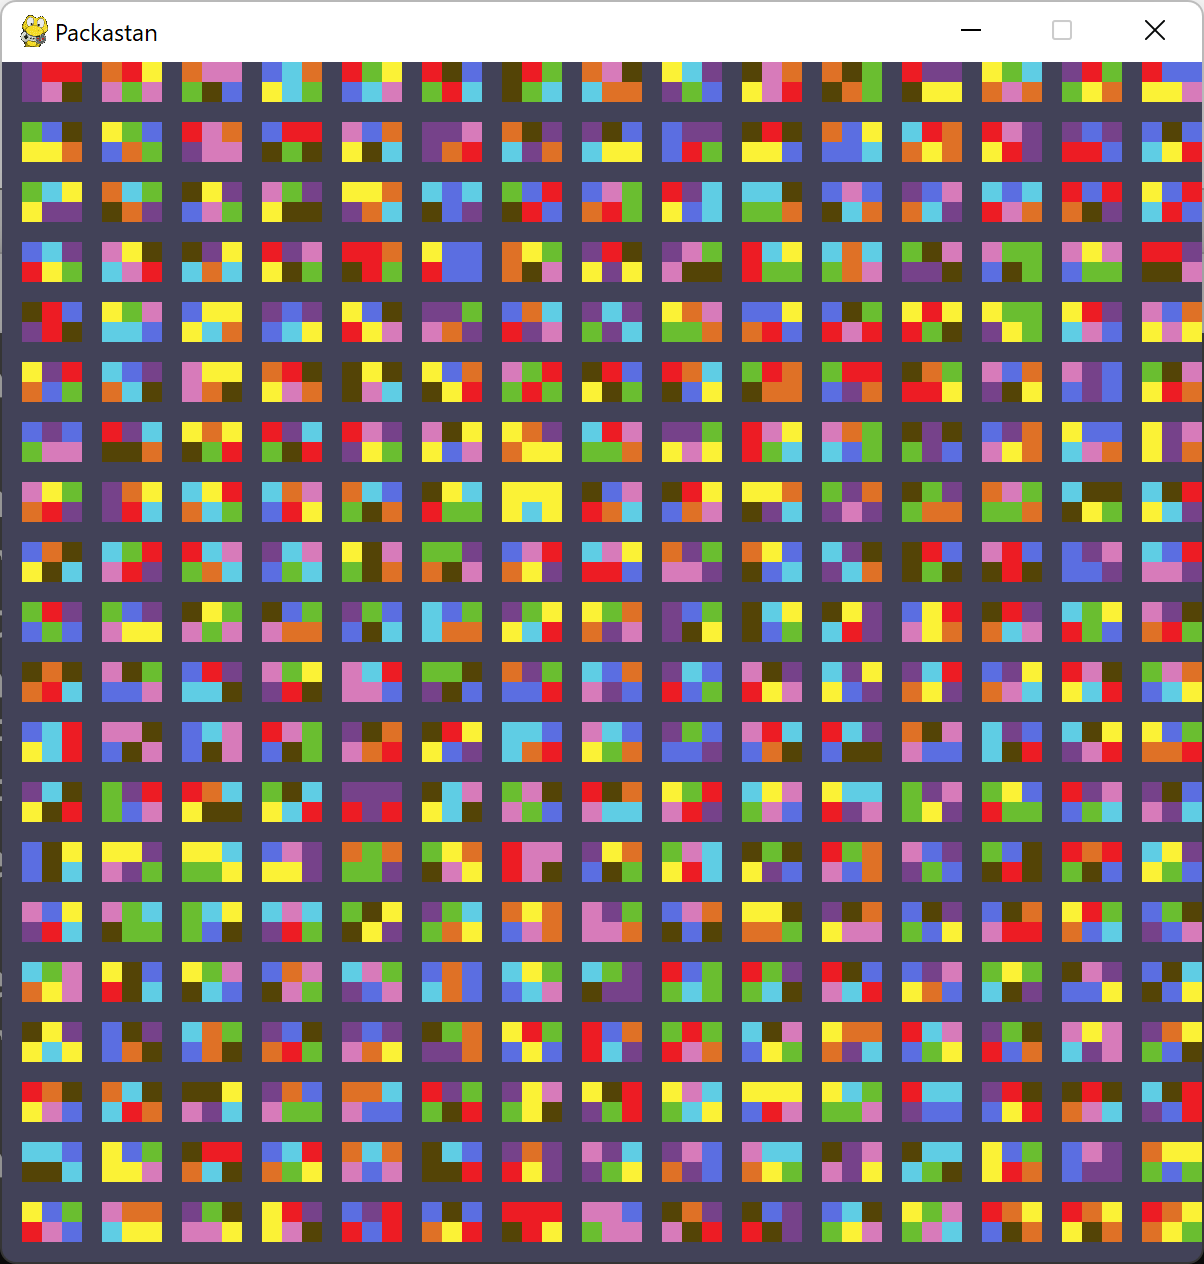
\includegraphics[scale=0.175]{diapo/Fig02.png}
        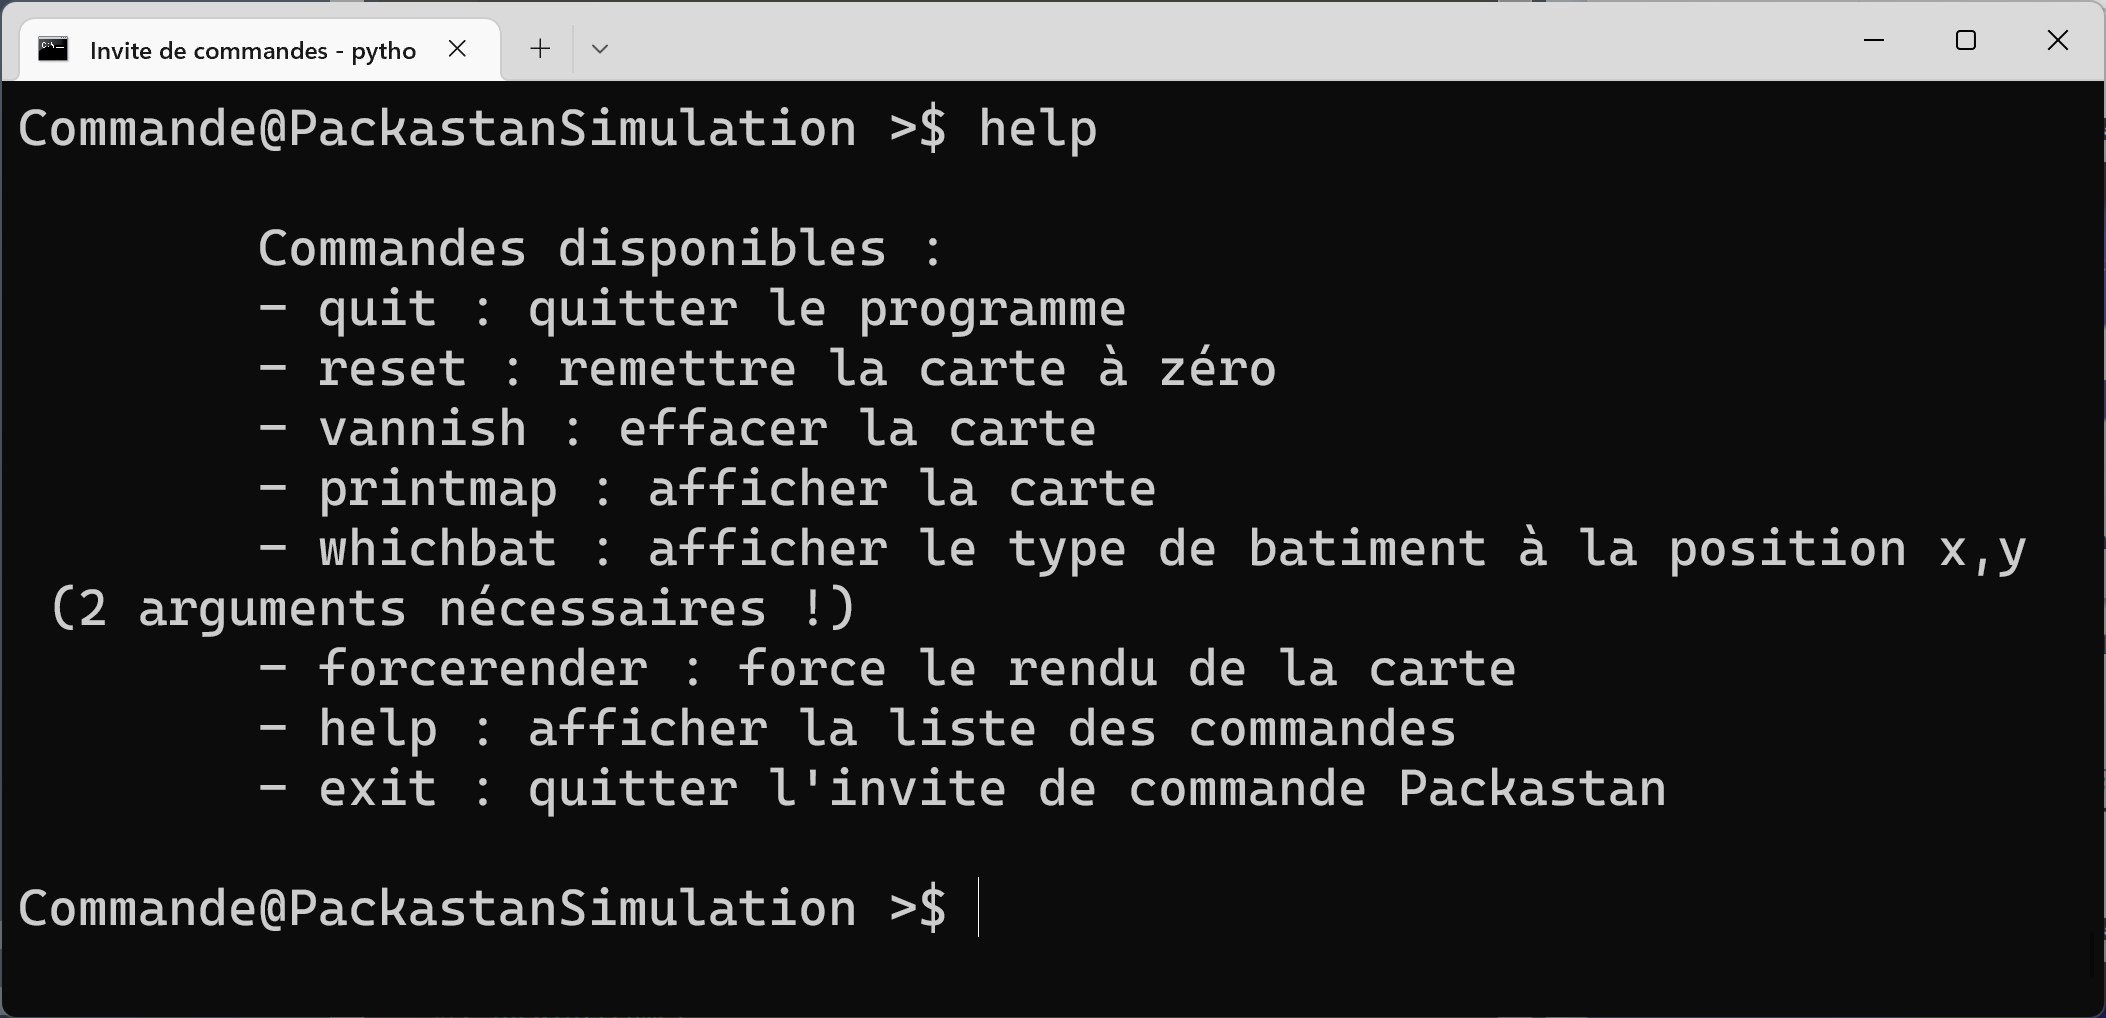
\includegraphics[scale=0.2]{diapo/Fig01.png}
    \end{center}
\end{frame}


%%%%%%%%%%%%%%%%%%%%%%%%%%%%%%%%%%%%%%%%%%%%%%%%
% Deuxième diapo
%%%%%%%%%%%%%%%%%%%%%%%%%%%%%%%%%%%%%%%%%%%%%%%%
\begin{frame}
	\frametitle{Affichage et interface avec la modélisation}
	\framesubtitle{Implémentation d'un moteur de modélisation : \texttt{pygame}}

	\begin{block}{Principe de fonctionnement}
	    \pause
        \begin{itemize}
            \item Une classe \texttt{Game} : \begin{itemize}
                \item Gestion du temps
                \item Position et instanciation des bâtiments
            \end{itemize}
            \pause
            \item Une classe \texttt{Tilemap} : \begin{itemize}
                \item \textit{Grille} à proprement parler
                \item Représente la grille comme un \texttt{n-domensional array} de la librairie \texttt{numpy}
            \end{itemize}
            \pause
            \item Une classe \texttt{Tileset} : \begin{itemize}
                \item Lie le type de bâtiment avec une ressource graphique (ici une couleur)
                \item Attribue un \textit{id} de bâtiment à chaque type ($\rightarrow$ cf. classe \texttt{Batiment})  
            \end{itemize}
        \end{itemize}
	\end{block}
\end{frame}

%%%%%%%%%%%%%%%%%%%%%%%%%%%%%%%%%%%%%%%%%%%%%%%%
% Troisième diapo
%%%%%%%%%%%%%%%%%%%%%%%%%%%%%%%%%%%%%%%%%%%%%%%%
\begin{frame}
	\frametitle{Affichage et interface avec la modélisation}
	\framesubtitle{Rendu de la visualisation}

\begin{figure}
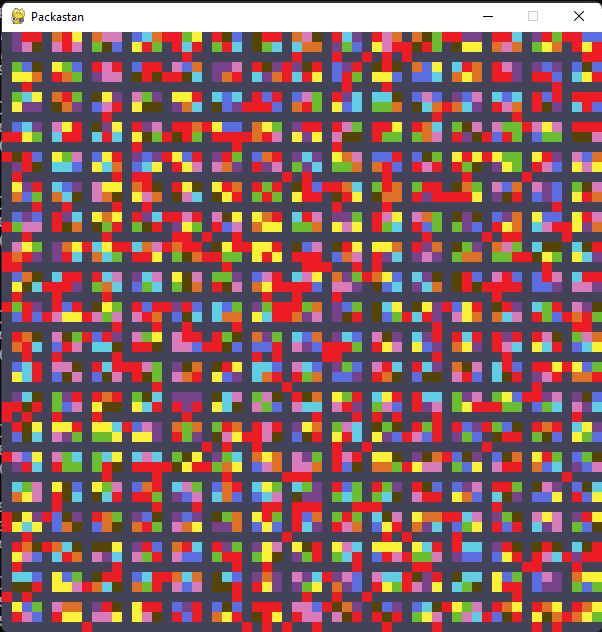
\includegraphics[scale=.4]{diapo/Fig03.png}
\end{figure}

\end{frame}

%%%%%%%%%%%%%%%%%%%%%%%%%%%%%%%%%%%%%%%%%%%%%%%%
% Quatrième diapo
%%%%%%%%%%%%%%%%%%%%%%%%%%%%%%%%%%%%%%%%%%%%%%%%
\begin{frame}
	\frametitle{Affichage et interface avec la modélisation}
	\framesubtitle{Interface via le \texttt{shell}}
    Principe de fonctionnement : 
    \pause
    \begin{exampleblock}{Appel}
        Interrompre l'exécution de la simmulation via une touche au clavier
    \end{exampleblock}
    \pause
    \begin{block}{Ajout et implémentation de fonctions}
        Pouvoir appeler des fonctions stockées dans un dictionnaire dans la classe principale, éventuellement avec des arguments
    \end{block}
    \pause
    \begin{alertblock}{Capacités d'action}
        Possibilités de \textit{récupérer} des données mais aussi d'en \textit{injecter} pendant le \textit{runtime}
    \end{alertblock}
 
\end{frame}
